% !TEX root SCHISADCJPOA JPFDÈOC KJ+ÒLDkc= ../Thesis.tex

\chapter{tecniche per la fusione di immagini SAR despeckled}
Per la fusione delle immagini denoised prodotte da differenti modelli di despeckling sono state esplorate varie strategie.
In una fase iniziale è stata adottata una tecnica naive, basata su un’architettura U-Net, in cui vengono addestrati 
tanti modelli quanti sono i metodi di despeckling considerati.
Ciascun modello ha il compito di apprendere a prevedere la qualità del proprio output denoised, generando così mappe 
di qualità che indicano, per ogni regione dell’immagine, quanto contributo includere da ciascun modello in 
base alla bontà del risultato ottenuto.
Per valutare l’efficacia di questa strategia, i risultati ottenuti sono stati confrontati con quelli derivanti 
da una fusione mediante semplice media aritmetica tra le immagini denoised, al fine di verificare se 
la previsione della qualità apportasse un reale miglioramento alla qualità visiva e strutturale dell’immagine finale.
L’approccio proposto in \cite{li2024crossfuse} introduce meccanismi di attenzione incrociata (cross-attention), 
che consentono una fusione più coerente e informata tra le diverse rappresentazioni delle immagini.
A differenza delle tecniche tradizionali, che attribuiscono pesi ai singoli pixel, questi metodi prevedono 
l’estrazione di feature dai vari output despeckled e l’impiego di un modulo di attenzione per selezionare, 
a livello di caratteristiche e di contesto, quali informazioni mantenere e quali attenuare.
Tale metodologia è stata originariamente concepita per la fusione di dati provenienti da domini eterogenei, 
come immagini ottiche e infrarosse, e include meccanismi per enfatizzare i dettagli complementari tra i diversi input.
L’approccio basato su patch consente di superare i limiti delle fusioni pixel-wise, poiché permette di catturare informazioni 
contestuali e di valorizzare le relazioni strutturali presenti nell’immagine.
Operando su blocchi di feature piuttosto che su pixel isolati, il modello è in grado di preservare meglio i bordi e le 
discontinuità, garantendo una maggiore coerenza spaziale e riducendo il rischio di smussare i contorni netti.
A partire da questi presupposti, è stata infine esplorata una tecnica alternativa che adotta un modello più semplificato 
e specifico per il dominio SAR.
In questo caso, il modello prende in input esclusivamente immagini appartenenti allo stesso dominio, concentrandosi 
non più sull’enfatizzazione delle caratteristiche complementari, ma sull’estrazione e valorizzazione 
delle caratteristiche comuni tra i diversi output denoised.
Questa scelta riduce la complessità architetturale e rende la fusione più efficace e coerente con l’obiettivo del 
lavoro, ossia migliorare la qualità complessiva dell’immagine despeckled nel contesto SAR.


\section{Dataset}

Come illustrato in Figura \ref{fig:MockReteNeurale}, il dataset impiegato è costituito da tre tipologie di 
immagini: clean, noisy e denoised tutte e tre ad un canale, ovvero in scala di grigi. Queste immagini sono state realizzate tramite uno strumento ottico di un
satellite per poi essere sporcate con speckle artificiale e su cui infine è stato fatto denoising. Questa scelta è stata fatta 
per poter avere sia l'immagine clean che quella noisy, fondamentali per gli eddestramenti supervisionati. Inoltre 
risulta difficile reperire un dataset contenenti immagini SAR comprese di ground truth abbastanza grandi da poter essere utlizzati per 
addestrare una rete neurale. Le immagini su cui viene fatto l'addestramento sono relative ad un singolo modello di despeckling ed ad 
un determinato look. Quest'ultimo è una metrica che indica l'intensità dello speckle artificiale, in quanto a più look,
corrispondono più catture di quella che è la realtà di interesse e quindi si ha una maggior precisione e uno speckle ridotto.


\section{Approccio basato sulla previsione della qualità}
\subsection{Manipolazione del dataset pre addestramento}
Le immagini prima di essere passate alla rete vengono normalizzate nell'intervallo $[0,1]$.
In fase di addestramento, le immagini noisy e denoised vengono concatenate in un unico tensore a due dimensioni e utilizzate come 
input per la rete neurale. Le immagini clean $[\hat{I}]$, invece, assieme a quelle denoised $[I]$, vengono impiegate per la 
generazione della mappa di qualità $[QM]$, che costituisce il riferimento necessario per 
il calcolo della funzione di loss. Questa mappa viene generata facendo la diffrenze in valore assoluto delle due immagini:
\begin{equation}
  \makebox[\textwidth][c]{%
    $\displaystyle
      QM = |\hat{I} - I |
    $%
  }
\end{equation}
Questo permette al modello di imparare a 
prevedere la qualità del denoising relative ad un dato modello di despeckling e ad una determinata intensità dello speckle. 
\begin{figure}[H]
    \centering
    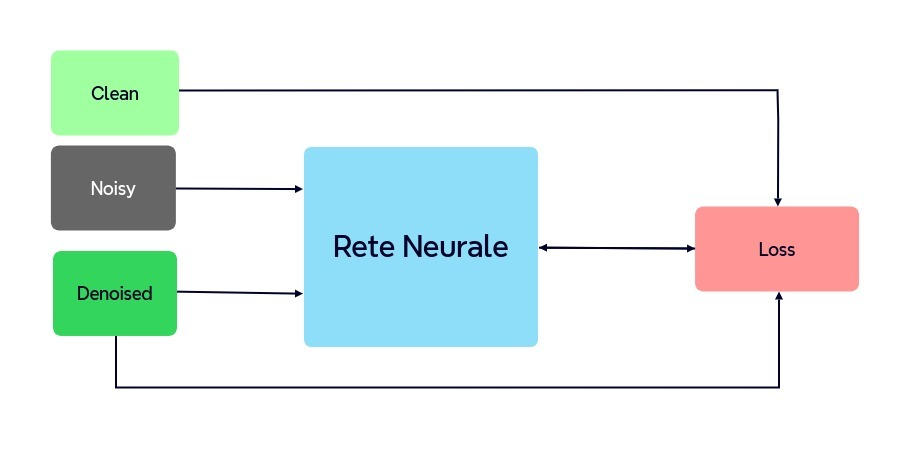
\includegraphics[width=0.8\textwidth]{utils/Architettura_rete_neurale.jpg}
    \caption{Mock della struttura logica per la previsione della qualità}
    \label{fig:MockReteNeurale}
\end{figure}

\section{Architettura rete neurale}
Come architettura della rete neurale è stata utilizzata la Unet. Questo perchè risulta particolarmente adatto per la 
generazione di una mappa di qualità che valuti l'affidabilità di un'immagine sottoposta a denoising \cite{Vyver2025}. che trattano dell'argomento. Il compito di 
questa rete è assegnare a ciascun pixel un valore compreso nell'intervallo $[0,1]$ che ne rappresenti la 
qualità locale. Questo output per la sua natura richiede un'architettura in grado di produrre una mappa di densità 
della stessa risoluzione spaziale dell'input, preservando la localizzazione precise delle informazioni. 
L'architettura \cite{ronneberger2015unetconvolutionalnetworksbiomedical}, è composta da due parti principali: encoder e decoder. 
Encoder, ovvero una sequenza di blocchi convoluzionali e operazioni di pooling che estraggono feature 
gerarchiche via via più astratte, consentendo alla rete di catturare il contenuto semantico dell’immagine, 
distinguere texture, bordi e regioni omogenee, e modellare la natura statistica del rumore.
Decoder, una fase simmetrica che ricostruisce progressivamente la risoluzione spaziale 
mediante up-sampling e convoluzioni, trasformando le feature ad alto livello in una mappa di 
qualità densa e dettagliata.
Elemento distintivo della U-Net sono le skip connections, che collegano i livelli dell’encoder ai corrispondenti 
livelli del decoder. Questi collegamenti trasferiscono mappe di feature ad alta risoluzione direttamente al decoder, 
preservando l’informazione spaziale fine indispensabile per localizzare correttamente dettagli critici come bordi 
sottili e piccole texture. Senza tali connessioni, il decoder produrrebbe output più sfocati, perdendo la capacità 
di discriminare le aree più sensibili agli artefatti di oversmoothing o agli errori di ricostruzione.
\begin{figure}[H]
  \centering
  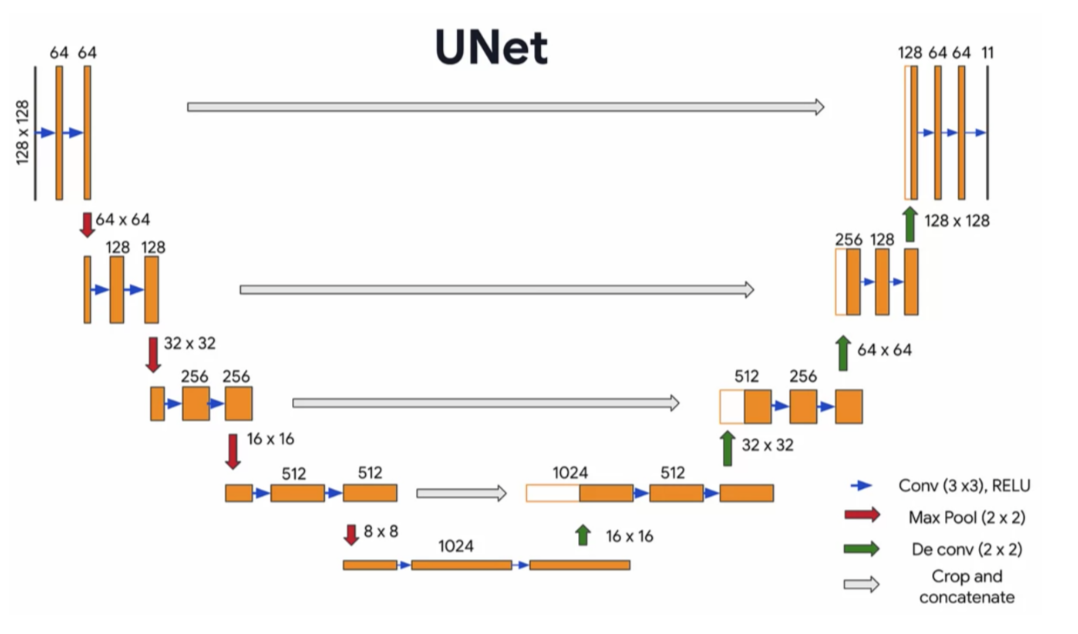
\includegraphics[width=\textwidth]{utils/unet.png}
  \caption{Architettura Unet}
  \label{fig:ArchitetturaUnet}
\end{figure}
L’aspetto più importante di questo modello è la sua capacità di andare oltre una semplice misura di errore pixel-wise. 
La rete apprende a sviluppare una vera e propria percezione semantica dell’errore, cioè a valutare la gravità di una 
discrepanza in funzione del contesto visivo in cui compare. Ad esempio, un errore di grande entità in una regione 
uniforme (come un cielo sereno) è visivamente più disturbante di un errore di pari entità in una regione altamente 
texturizzata (come del fogliame), dove può essere facilmente mascherato. Analogamente, un piccolo errore su un bordo 
netto è percettivamente rilevante. L’encoder, stratificando feature di complessità crescente, apprende questa gerarchia 
di contenuti visivi e fornisce al decoder le informazioni necessarie per produrre una mappa di qualità che pondera 
ogni errore in base alla sua importanza percettiva.

\section{Fusione dei modelli}
La fusione delle immagini denoised $[I]$ prodotte tramite i rispettivi modelli di despeckling vengono fusi attraverso una media pesata sfuttando
le mappa di qualità $[M]$ come pesi per le singole immagini.
\begin{equation}
    \makebox[\textwidth][c]{%
      $\displaystyle
        \frac{\sum_{i=1}^{n} I_i M_i}{\sum_{i=1}^{n} M_i}
      $%
    }
\end{equation}
È un processo che si comporta in modo diverso per ogni singolo pixel dell'immagine. Se il Modello A ha una qualità stimata 
molto alta in una regione e il Modello B molto bassa, la fusione privilegerà maggiormente 
il Modello A in quella determinata area. Mentre alcuni sono eccellenti nel preservare i bordi netti ma possono lasciare del rumore residuo nelle aree lisce, 
altri sono ottimi nell' eliminare il rumore dalle superfici lisce ma tendono a sfocare (oversmooth) i bordi e le texture.
La fusione pesata permette di prendere il meglio di ogni modello usando di più l'output dell'algoritmo migliore per una data 
caratteristica dell'immagine, e meno i suoi contributi peggiori.
\\\\
\section{Funzione di loss}
Come funzione di perdità è stata utilizzata la mean square error [MSE] tra l'output della fusione [I] 
e il ground truth [$\hat{I}$], ovvero l'immagine clean . 
\begin{equation}
  \makebox[\textwidth][c]{%
    $\displaystyle
    \text{MSE} = \left( I - \hat{I} \right)^2
    $%
  }
\end{equation}
Questa funzione di perdità è stata scelta in quanto è molto facile da calcolare eccellenti 
non presenta particolari complicazioni in fase di ottimizzazzione. Inoltre 
dato che PSNR è funzione del MSE, ottimizzare la MSE porta anche ad avere valori 
più alti di PSNR, che spesso viene usato come metrica di valutazione 

\section{Limiti dei questa tecnica}
Sebbene la media pesata presenti il vantaggio di combinare in maniera coerente i contributi dei vari modelli di despeckling, 
essa introduce alcune criticità che ne riducono l’efficacia in scenari complessi.
In primo luogo, la media pesata tende a diluire i dettagli sottili. Se una delle immagini denoised contiene strutture fini 
o bordi ben preservati che altre non hanno, questi dettagli possono risultare attenuati o addirittura persi, poiché la 
media li combina con le versioni più lisce prodotte dagli altri modelli. Ciò porta a un effetto di oversmoothing, che riduce 
il livello di dettaglio complessivo dell’immagine fusa.
Un’ulteriore limitazione deriva dal fatto che la media pesata opera pixel per pixel, senza considerare la correlazione spaziale 
tra pixel adiacenti. Pattern, texture e strutture complesse che sono distribuite su più pixel non vengono trattati in maniera 
coerente. Questo può portare a artefatti locali, soprattutto ai bordi o in aree con pattern ripetitivi, dove una decisione 
puramente puntuale può introdurre discontinuità.
Inoltre, se il rumore è altamente non stazionario o presenta componenti strutturate, la rete che genera le mappe di qualità 
può faticare a distinguere tra rumore residuo e dettaglio fine. In queste situazioni la mappa di qualità può risultare 
inaccurata, assegnando un peso elevato a regioni che in realtà presentano artefatti o penalizzando aree visivamente corrette. 
Questo porta a una fusione non ottimale, che può accentuare il rumore residuo o degradare regioni già ben restaurate.
Va considerato anche il problema della sensibilità agli errori di predizione della mappa di qualità. Poiché i pesi influenzano 
direttamente il risultato finale, eventuali errori nella stima della qualità si traducono in artefatti amplificati nell’immagine 
fusa, specialmente se un singolo modello viene sovrastimato in regioni dove la sua qualità non è affidabile.

\section{Approccio basato sulla self e cross attention}
Usare un approccio basato sulla self e cross attention permette di effettuare la fusione non basandosi su una strategia 
pixel per pixel ma su patch, ovvero 
una piccola regione localizzata o un sottoinsieme di pixel all'interno di 
un'immagine più grande, in genere rettangolare o quadrata.
L’obiettivo del meccanismo di fusione basato su self e cross attention è combinare 
in modo intelligente più immagini despeckled provenienti da diverse acquisizioni o canali per ottenere un’immagine finale più informativa, pulita e coerente. 
Per affrontare questa problematica, l’approccio proposto in \cite{li2024crossfuse} introduce un meccanismo di fusione basato su self e cross attention, ispirato ai modelli 
transformer, in grado di individuare e valorizzare le componenti informative complementari tra le immagini despeckled, riducendo al contempo la ridondanza residua.
In \cite{li2024crossfuse} mostra che una 
fusione che usa blocchi di self-attention per rinforzare le caratteristiche intra-modalità  
e una cross-attention progettata per esaltare le informazioni non correlate tra le modalità, produce immagini 
fuse con più dettaglio e con meno artefatti, migliorando le strutture rispetto a metodi più semplici. 
Il paper sottolinea inoltre che, in multimodal fusion, la cosa cruciale è valorizzare l’uncorrelation (cioè la complementarità) tra le modalità, 
cosa che la cross-attention è progettata per fare. Questo permette di combinare 
informazioni provenienti da regioni diverse e di differenti modalità, non solo di sommare pixel con pesi locali. 
Il metodo si fonda su una architettura ibrida composta da due blocchi principali.

\subsection{Self-Attention e Cross-Attention}
La self-attention è un meccanismo introdotto originariamente nei Transformer per consentire a 
una rete di mettere in relazione diverse parti dello stesso input tra loro, pesandole in base alla loro importanza reciproca.
Questo è diverso dalle convoluzioni (CNN) tradizionali, che analizzano solo piccole regioni locali, la self-attention, invece, 
cattura dipendenze globali, anche tra punti molto distanti dell’immagine. La cross-attention \cite{vaswani2023attentionneed} invece 
è un meccanismo di attenzione che permette a una sequenza di query provenienti da una sorgente 
(ad esempio un decoder) di pesare gli elementi di un’altra sequenza, da cui provengono le key e le value (ad esempio l’encoder).
In altre parole, essa modella le dipendenze incrociate tra due insiemi distinti di rappresentazioni.
\subsubsection{Funzionamento della Self-Attention}
Sia un'immagine despeckled \(I \in \mathbb{R}^{H \times W \times C}\), dove ogni patch può essere considerato come un token.  
Per ogni posizione \(i\) nell'immagine:

\begin{itemize}
    \item \textbf{Query \(Q_i\)}: rappresenta ciò che la posizione \(i\) sta cercando negli altri patch della stessa immagine.
    \item \textbf{Key \(K_j\)}: rappresenta le caratteristiche della posizione \(j\) che le altre posizioni possono usare per valutare la sua rilevanza.
    \item \textbf{Value \(V_j\)}: è l'informazione effettiva che la posizione \(j\) può trasmettere a \(i\).
\end{itemize}
Il pixel \(i\) può ``guardare'' altri pixel dell'immagine e decidere quali informazioni (ad esempio strutture, bordi, texture) prendere per migliorare la propria rappresentazione despeckled.

\subsubsection{Calcolo della Self-Attention}
Il primo passo consiste \cite{vaswani2023attentionneed} nel calcolare la similarità tra ogni Query della target e ogni Key della source, mediante un prodotto scalare:
\[
    \makebox[\textwidth][c]{%
      $\displaystyle
        Q \cdot K^T
      $%
    }
\]
Questo produce una matrice di dimensione $nxm$ in cui $n$ è il numero di elementi della target e $m$ 
quello della source. Ogni entry misura quanto un elemento della target “presta attenzione” a un elemento 
della source. Per stabilizzare la scala dei valori e prevenire problemi numerici, si divide per $\sqrt{d_k}$, ottenendo:
\[
    \makebox[\textwidth][c]{%
      $\displaystyle
        \frac{QK^T}{\sqrt{d_k}}
      $%
    }
\]
Successivamente, applichiamo la funzione softmax riga per riga, trasformando i punteggi in probabilità normalizzate. 
In questo modo, per ogni elemento della target otteniamo un insieme di pesi che indicano quanto ciascun elemento della source contribuisce alla rappresentazione finale:
\[
    \makebox[\textwidth][c]{%
      $\displaystyle
        \alpha = \text{softmax}\left(\frac{QK^T}{\sqrt{d_k}}\right)
      $%
    }
\]
Infine, la matrice dei pesi $\alpha$ viene moltiplicata per la matrice dei Value 
V, combinando le informazioni della source in modo ponderato e producendo i nuovi vettori rappresentativi per la target:
\begin{equation}
    \makebox[\textwidth][c]{%
      $\displaystyle
        \text{Attention}(Q, K, V) = \text{softmax}\left(\frac{Q K^\top}{\sqrt{d_k}}\right)V
      $%
    }
    \label{eq:attention}
    \end{equation}
    
\subsubsection{Differenza tra Self-Attention e  Cross-Attention}
L'attenzione viene calcolata come visto in \ref{eq:attention} con la differenza che nella cross-attention 
le matrici \(Q\), \(K\) e \(V\) provengono da sorgenti diverse. 
\begin{itemize}
  \item \textbf{Query \(Q\)}: proiezione lineare delle rappresentazioni del decoder
  \item \textbf{Key \(K\)}, \textbf{Value \(V\)}: proiezioni lineari delle rappresentazioni del encoder
\end{itemize}
In \cite{li2024crossfuse} la cross attention è il cuore del metodo di fusione. Il suo scopo principale non è, come nei transformer 
classici, massimizzare la correlazione tra due insiemi di feature, ma enfatizzare le informazioni complementari 
(cioè non correlate) tra immagini visibile e infrarossa.

\subsection{Architettura del modello}
Due encoder (con la stessa struttura ma parametri diversi) estraggono le feature rispettivamente dall’immagine infrarossa (IR) e visibile (VI), 
servono per catturare le caratteristiche specifiche di ciascuna modalità. Le feature di ciascun encoder passano prima attraverso blocchi di 
self-attention (SA) per migliorare la coerenza intra-modale (dettagli e struttura interna all’immagine).
Poi interviene il Cross-Attention Mechanism (CAM), dove avviene la fusione vera e propria tra le due modalità.
Il decoder ricostruisce l’immagine fusa a partire dalle feature integrate dal CAM, con skip connection per preservare dettagli e salienza.
\subsubsection{Cross-Attention Mechanism}
Il CAM combina self-attention e cross-attention in modo da: potenziare le intra-feature di ciascuna modalità; evidenziare le inter-feature complementari tra IR e VI.
Ogni modalità entra in una catena di blocchi:
\begin{figure}[H]
  \centering
  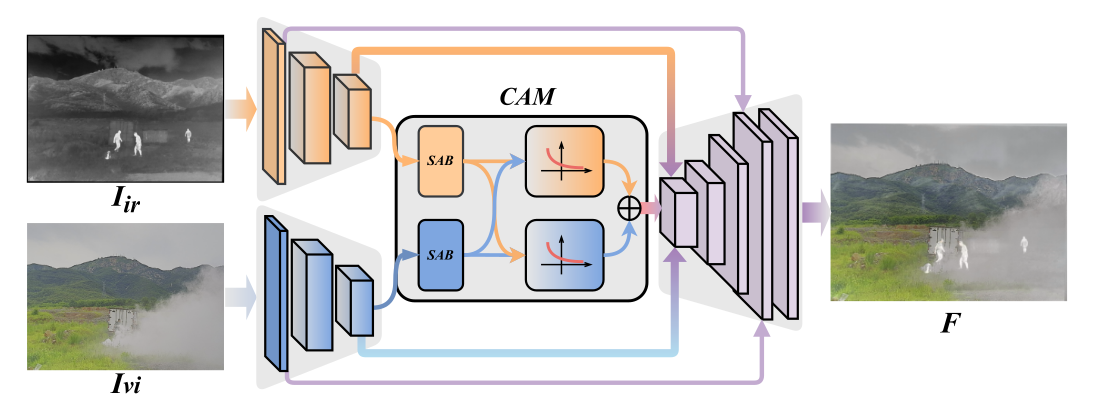
\includegraphics[width=1.0\textwidth]{utils/blocchi.png}
  \caption{I due Encoder hanno la stessa architettura ma parametri differenti. 
  Il meccanismo di cross-attention (CAM) viene utilizzato per fondere le caratteristiche multimodali. 
  “SAB” indica il blocco di self-attention. L’immagine fusa può essere ottenuta tramite il Decoder, 
  che include una connessione lunga proveniente dagli encoder.}
  \label{fig:blocchi}
\end{figure}
I due blocchi di Self-Attention (SA) servono a rafforzare le caratteristiche interne.
L’operazione di Shift/Unshift sposta e ripristina le feature, per aumentare la copertura spaziale globale.
Il Cross-Attention (CA) è il passo cruciale, che integra le due modalità.
\subsubsection{Reversed Softmax}
Il cross-attention è calcolato come nel transformer standard, ma con una differenza fondamentale:
\[
    \makebox[\textwidth][c]{%
      $\displaystyle
        \text{re-softmax(X) = softmax(-X)}
      $%
    }
\]
Questo significa che: invece di dare peso alto alle feature simili (correlate) come fa il softmax classico, 
la re-softmax dà peso alto alle feature dissimili (non correlate). 
CAM enfatizza ciò che una modalità ha e l’altra no, ossia l’informazione complementare, che è essenziale per la fusione

\subsection{Fusione dei modelli}
Nel caso della fusione si hanno quattro autoencoder, ciascuno dedicato a una diversa rappresentazione dell’immagine SAR (SAR-CAM, FANS, SARBM3D, noisy).
Ciò estende il principio di CrossFuse da una fusione bimodale a una 
fusione multimodale. L’idea alla base rimane la stessa: combinare più sorgenti che condividono la stessa struttura spaziale ma presentano contenuti 
informativi parzialmente diversi o complementari, al fine di produrre un’immagine finale più completa, bilanciata e informativa.
Il punto di partenza del sistema è costituito dai quattro encoder, ognuno dei quali apprende a rappresentare la propria modalità secondo il 
suo dominio specifico. Le versioni despeckled prodotte con SARCAM, FANS e BM3D, pur avendo eliminato il rumore di tipo speckle, differiscono 
nel modo in cui trattano i dettagli fini e le strutture deboli: alcune tendono a privilegiare la continuità tonale, altre la preservazione 
dei bordi. L’immagine noisy, invece, pur essendo la più “sporca”, conserva informazione strutturale che spesso viene attenuata durante 
il despeckling. In questo contesto, gli encoder agiscono come estrattori di caratteristiche complementari: ciascuno mappa la propria immagine 
in uno spazio di rappresentazione latente dove si preservano sia i pattern condivisi (ad esempio, i contorni principali) sia le particolarità 
proprie del metodo di despeckling.
Una volta estratte le feature dalle quattro reti, la fusione non può limitarsi a un semplice concatenamento o media ponderata. È qui che 
entra in gioco la cross-attention. Invece di gestire due 
rami (come nel caso infrarosso-visibile), il modello deve essere capace di trattare interazioni multiple, valutando quanto ogni rappresentazione 
contribuisca alla formazione di un contenuto informativo unico. Ogni coppia di modalità può essere posta in relazione attraverso una cross-attention, 
dove la re-softmax viene applicata per enfatizzare la dissimilarità: in questo modo le componenti ridondanti, cioè le parti in cui le 
varie versioni coincidono, vengono attenuate, mentre le parti complementari, presenti solo in uno dei canali, vengono esaltate.
Il passo successivo consiste nel combinare queste diverse mappe di attenzione in una rappresentazione fusa. Questo può essere fatto in modo 
gerarchico, ad esempio con una attention aggregation layer, che raccoglie i risultati delle cross-attention tra le varie coppie di encoder e 
li integra progressivamente. In questo modo si costruisce un’unica mappa di caratteristiche latenti che racchiude i dettagli fini dei vari modelli, 
e riduce al minimo la ridondanza informativa.
Il decoder, a questo punto, ha il compito di ricostruire l’immagine finale partendo da questa rappresentazione fusa. 
Dal punto di vista concettuale, questa architettura si comporta come un “mediatore intelligente” tra diverse visioni dello stesso segnale: non 
sceglie a priori quale metodo di despeckling sia migliore, ma apprende a ponderare dinamicamente l’informazione proveniente da ciascuno in base 
alla sua unicità. La cross-attention, con la re-softmax, garantisce che il modello privilegi la diversità informativa invece della somiglianza, 
rendendo possibile una fusione realmente complementare e non una semplice media delle soluzioni.

\section{Semplificazione del modello CrossFuse}
Il modello CrossFuse nasce con l’obiettivo di affrontare un problema tipico della fusione multimodale tra immagini provenienti da 
domini diversi, in particolare ottico e infrarosso. In questi casi, i due sensori catturano informazioni complementari: l’immagine 
visibile contiene ricchezza di texture e colore, mentre quella infrarossa evidenzia le sorgenti di calore e le strutture non 
visibili a occhio nudo. Il compito della rete è quindi combinare tali informazioni massimizzando la complementarità e 
minimizzando la ridondanza tra le due modalità. Durante le spierimentazioni della tesi pero si è notato che,
tuttavia, se consideriamo il caso di immagini provenienti dallo stesso dominio, come due immagini ottiche acquisite in condizioni 
diverse o due versioni degradate di uno stesso contenuto, la situazione cambia profondamente.
In questo scenario, le informazioni di partenza non sono complementari ma ridondanti: la sfida non è più quella di mettere in evidenza 
le differenze tra domini, ma piuttosto di fondere in modo coerente informazioni simili, eliminando il rumore e preservando i dettagli condivisi.
Di conseguenza, molti dei meccanismi complessi introdotti in CrossFuse, come la doppia attenzione incrociata, il re-softmax o la doppia fase di addestramento, 
possono risultare superflui o addirittura controproducenti.
\begin{figure}[H]
  \centering
  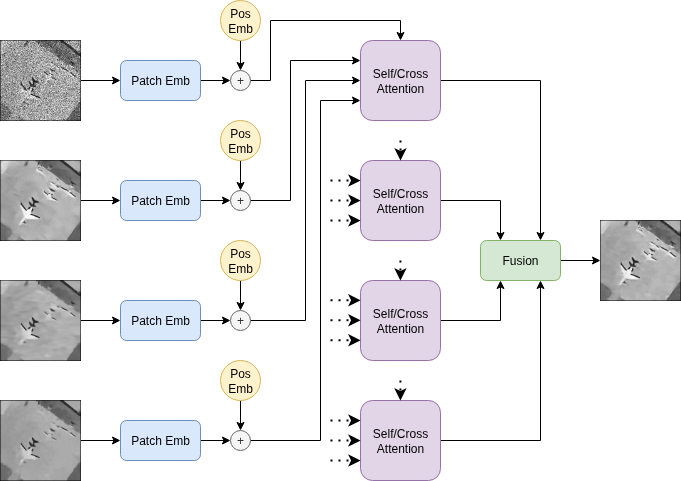
\includegraphics[width=1.0\textwidth]{utils/schema.png}
  \caption{Schema semplificato.}
  \label{fig:schema}
\end{figure}
Si parte da più immagini di input che appartengono allo stesso dominio.
Ogni immagine viene divisa in patch e passata attraverso un Patch Embedding , poi si aggiunge un Positional Embedding per mantenere l’informazione spaziale.
Le rappresentazioni ottenute passano attraverso una serie di blocchi di attenzione, indicati come “Self/Cross Attention” che possono modellare sia le relazioni interne all’immagine (self-attention) sia tra immagini (cross-attention).
Infine, le feature elaborate vengono combinate in un modulo di Fusion, che produce l’immagine fusa finale.
CrossFuse cerca l’informazione mancante nell’altro dominio, la versione semplificata cerca l’informazione comune e più stabile tra immagini simili.
Per questo motivo, eliminare meccanismi come il re-softmax o la doppia fase di addestramento, nati per gestire la non-correlazione 
può non solo semplificare l’architettura, ma anche migliorare le prestazioni nei contesti monomodali.

% !TEX root = ../Thesis.tex


 

